\begin{figure}
	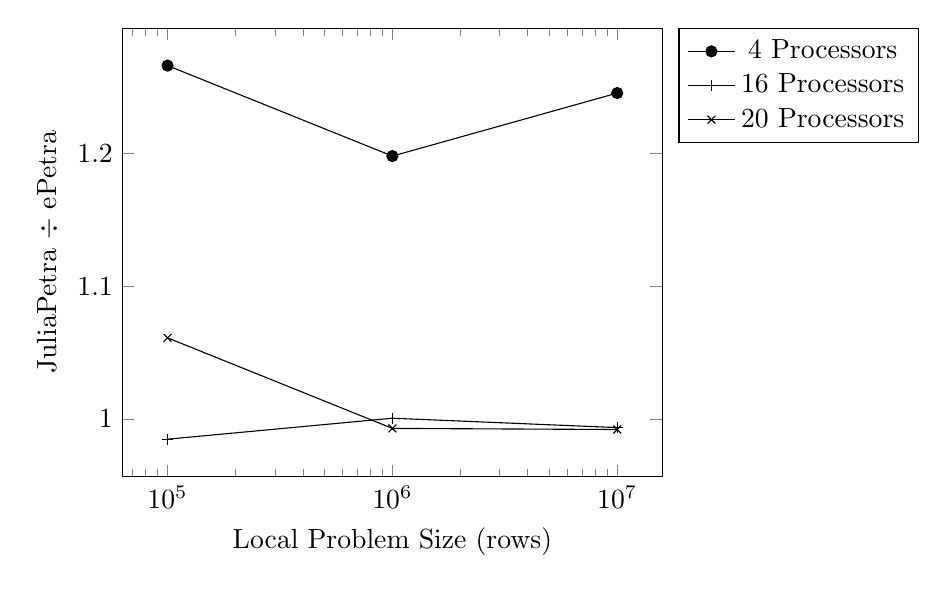
\begin{tikzpicture}
		\begin{axis}[
		        xmode=log,
		        xlabel={Local Problem Size (rows)},
		        ylabel = {JuliaPetra \(\div\) ePetra},
		        legend pos = outer north east
		    ]
			\addplot[color=black,mark=*] coordinates{(100000,1.26633)(1000000,1.19812)(10000000,1.24562)};
			\addlegendentry{4 Processors}
			\addplot[color=black,mark=+] coordinates{(100000,0.98474)(1000000,1.00055)(10000000,0.99348)};
			\addlegendentry{16 Processors}
			\addplot[color=black,mark=x] coordinates{(100000,1.06114)(1000000,0.99287)(10000000,0.99204)};
			\addlegendentry{20 Processors}
		\end{axis}
	\end{tikzpicture}
	\caption{Problem Size Versus JuliaPetra \(\div\) ePetra}
\end{figure}

\begin{figure}
	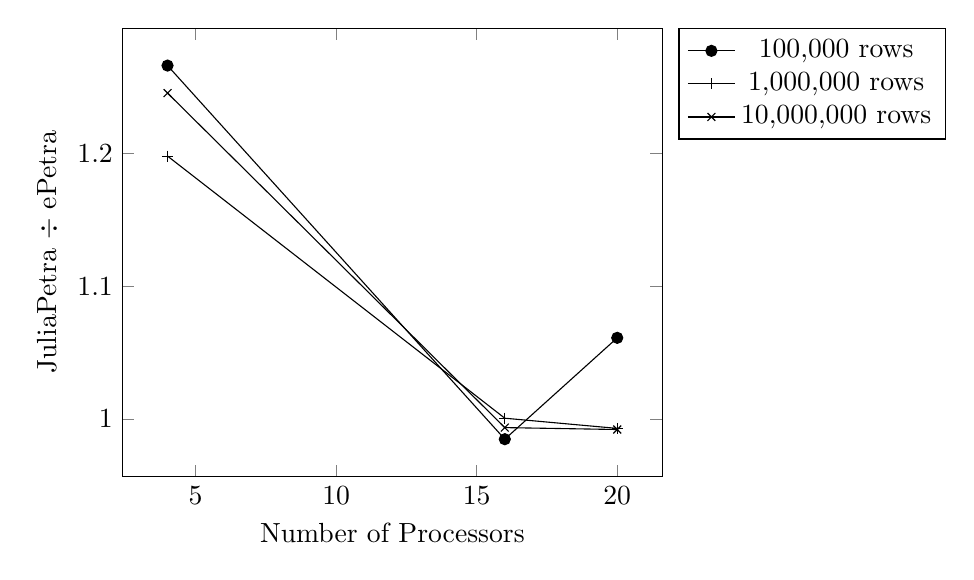
\begin{tikzpicture}
		\begin{axis}[
		        xlabel = {Number of Processors},
		        ylabel = {JuliaPetra \(\div\) ePetra},
		        legend pos = outer north east
		    ]
			\addplot[color=black,mark=*] coordinates{(4,1.26633)(16,0.98474)(20,1.06114)};
			\addlegendentry{100,000 rows}
			\addplot[color=black,mark=+] coordinates{(4,1.19812)(16,1.00055)(20,0.99287)};
			\addlegendentry{1,000,000 rows}
			\addplot[color=black,mark=x] coordinates{(4,1.24562)(16,0.99348)(20,0.99204)};
			\addlegendentry{10,000,000 rows}
		\end{axis}
	\end{tikzpicture}
	\caption{Number of Processors Versus JuliaPetra \(\div\) ePetra}
\end{figure}
